% Source problem: https://www.ap.t.u-tokyo.ac.jp/themes/ap_t_u-tokyo/graduate/pdf/h26ap_exam.pdf
\documentclass[11pt,a4paper]{article}
\usepackage[margin=23mm]{geometry}
\usepackage{fontspec}
\usepackage{xeCJK}
\setCJKmainfont{HaranoAjiMincho-Regular.otf}
\setCJKsansfont{HaranoAjiGothic-Medium.otf}
\usepackage{amsmath,amssymb}
\usepackage{tikz}
\setlength{\parindent}{1em}
\setlength{\parskip}{0.35em}
\title{物理工学専攻 院試解答集\\2014年度 物理学II 第1問}
\author{政岡凜太郎}
\date{}
\begin{document}
\maketitle

\section*{[1] Pauli行列の固有状態}
$|\alpha\rangle=(1,0)^T$, $|\beta\rangle=(0,1)^T$ を $\sigma_z$ の固有値 $+1,-1$ の状態とする。行列の作用を直接計算すると
\begin{align}
 \sigma_x\frac{|\alpha\rangle+|\beta\rangle}{\sqrt2}
 &=+\frac{|\alpha\rangle+|\beta\rangle}{\sqrt2},&
 \sigma_x\frac{|\alpha\rangle-|\beta\rangle}{\sqrt2}
 &=-\frac{|\alpha\rangle-|\beta\rangle}{\sqrt2},\\
 \sigma_y\frac{|\alpha\rangle+i|\beta\rangle}{\sqrt2}
 &=+\frac{|\alpha\rangle+i|\beta\rangle}{\sqrt2},&
 \sigma_y\frac{|\alpha\rangle-i|\beta\rangle}{\sqrt2}
 &=-\frac{|\alpha\rangle-i|\beta\rangle}{\sqrt2}.
\end{align}
したがって $|\pm x\rangle=(|\alpha\rangle\pm|\beta\rangle)/\sqrt2$、$|\pm y\rangle=(|\alpha\rangle\pm i|\beta\rangle)/\sqrt2$ がそれぞれ固有値 $\pm1$ の規格化固有状態である。

\section*{[2] 電場中の一次元運動}
\subsection*{[2.1] ハミルトニアン}
$\boldsymbol p=p_x\boldsymbol e_x$, $\boldsymbol E=E\boldsymbol e_z$ なので $\boldsymbol p\times\boldsymbol E=-p_xE\boldsymbol e_y$。従って
\begin{equation}
 H=\frac{p_x^2}{2m}+H_{\rm SO}
 =\boxed{\frac{p_x^2}{2m}-\frac{\gamma E}{\hbar}p_x\sigma_y}.
\end{equation}

\subsection*{[2.2] 分散とスピン}
平面波 $\phi_k(x)=e^{ikx}$ では $p_x=\hbar k$ だから
\begin{equation}
 H(k)=\frac{\hbar^2k^2}{2m}-\gamma Ek\sigma_y.
\end{equation}
$\sigma_y$ 固有値を $s=\pm1$ とし、$|y,+1\rangle=|+y\rangle$、$|y,-1\rangle=|-y\rangle$ と書くと、固有関数と固有エネルギーは
\begin{align}
 \psi_{k,s}(x)&=e^{ikx}|y,s\rangle,\\
 E_s(k)&=\frac{\hbar^2k^2}{2m}-s\gamma Ek
 =\frac{\hbar^2}{2m}\left(k-\frac{sm\gamma E}{\hbar^2}\right)^2
  -\frac{m\gamma^2E^2}{2\hbar^2}.
\end{align}
二本は $k=0$ で交差する放物線で、それぞれの固有枝ではスピンは一定の $s\boldsymbol e_y$ を向く。$\gamma<0$ のため、各 $k\ne0$ で低い方の枝は $s=\operatorname{sgn}(\gamma k)=-\operatorname{sgn}(k)$ である。つまり最低エネルギー状態を $k<0$ から $k>0$ へ移るとスピンは $+y$ から $-y$ へ反転する。交差点 $k=0$ では縮退しており、スピン方向は一意に定まらない。

$k_*=|m\gamma E|/\hbar^2$、$E_*=m\gamma^2E^2/(2\hbar^2)$、$x=k/k_*$ と置けば $E_s/E_*=x^2+2sx$ である。分散を図示する。
\begin{center}
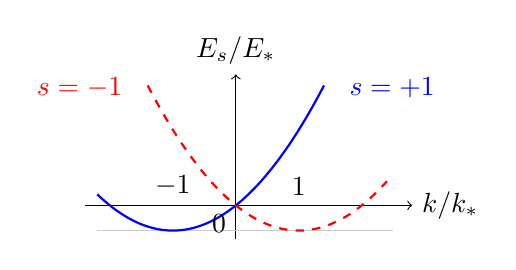
\begin{tikzpicture}[x=0.8cm,y=0.32cm]
 \draw[->] (-2.4,0)--(2.8,0) node[right] {$k/k_*$};
 \draw[->] (0,-1.35)--(0,5.2) node[above] {$E_s/E_*$};
 \draw[gray!40] (-2.2,-1)--(2.5,-1);
 \draw[thick,blue,domain=-2.2:1.4,samples=100] plot (\x,{\x*\x+2*\x});
 \draw[thick,red,dashed,domain=-1.4:2.4,samples=100] plot (\x,{\x*\x-2*\x});
 \draw[dotted] (0,-1.15)--(0,4.8);
 \node[blue,anchor=west] at (1.65,4.65) {$s=+1$};
 \node[red,anchor=east] at (-1.65,4.65) {$s=-1$};
 \node[below left] at (0,0) {$0$};
 \node[above] at (1,0) {$1$};
 \node[above] at (-1,0) {$-1$};
\end{tikzpicture}
\end{center}
青実線と赤破線は $\sigma_y$ の固有値 $+1,-1$ に対応する。放物線の頂点はそれぞれ $k/k_*=-1,+1$ にあり、エネルギーは $-E_*$ である。

\subsection*{[2.3] Zeeman場を加えた場合}
$\Delta=g\mu_BB/2>0$ とおくと、Zeeman項を含む運動量表示ハミルトニアンは
\begin{equation}
 H(k)=\frac{\hbar^2k^2}{2m}+\Delta\sigma_x-\gamma Ek\sigma_y
 =\frac{\hbar^2k^2}{2m}+\boldsymbol h(k)\cdot\boldsymbol\sigma,
 \qquad \boldsymbol h(k)=(\Delta,-\gamma Ek,0).
\end{equation}
Pauli行列の反交換関係から $(\boldsymbol h\cdot\boldsymbol\sigma)^2=|\boldsymbol h|^2I$ となり、$\boldsymbol h\cdot\boldsymbol\sigma$ の固有値は $\pm|\boldsymbol h|$ である。従って
\begin{equation}
 \boxed{E_\pm(k)=\frac{\hbar^2k^2}{2m}
 \pm\sqrt{\Delta^2+(\gamma Ek)^2}}.
\end{equation}
$k=0$ の準位差は $2\Delta=g\mu_BB$ で、電場のみの交差が有限の間隔を持つ反交差となる。その規格化固有状態で $\{\sigma_j,\boldsymbol h\cdot\boldsymbol\sigma\}=2h_jI$ の期待値を取ると、$2(\pm|\boldsymbol h|)\langle\sigma_j\rangle_\pm=2h_j$（$j=x,y,z$）である。従ってスピン期待値は
\begin{equation}
 \boxed{\langle\boldsymbol\sigma\rangle_\pm
 =\pm\frac{(\Delta,-\gamma Ek,0)}{\sqrt{\Delta^2+(\gamma Ek)^2}}.}
\end{equation}
よって $k=0$ では上枝が $+x$、下枝が $-x$ を向く。$\gamma<0$ なら $h_y=-\gamma Ek$ は $k$ と同じ符号を持つ。$|k|$ が大きくなるにつれて、上枝のスピンは有効場 $\boldsymbol h(k)$ と平行、下枝のスピンは反平行のまま連続的に回る。十分大きな正の $k$ では上枝が $+y$、負の $k$ では上枝が $-y$ に近づき、下枝は反対向きとなる。

固有エネルギーの概略は次のようになる。$q=k/k_0$, $k_0=\Delta/(|\gamma|E)$ とし、二次項の無次元係数 $c=\hbar^2k_0^2/(2m\Delta)$ を表示例として $c=1$ に選ぶ。したがって曲線は $E_\pm/\Delta=q^2\pm\sqrt{1+q^2}$ で、$q=0$ のギャップは $2\Delta=g\mu_BB$ である。曲率は $c$ に依存する。
\begin{center}
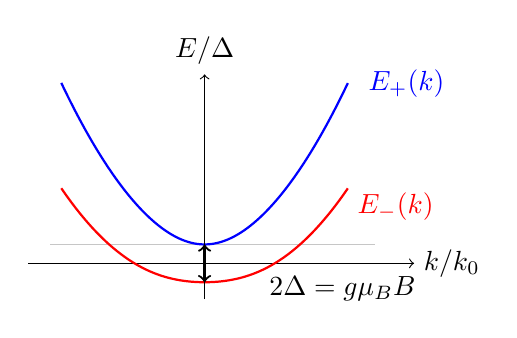
\begin{tikzpicture}[x=0.7cm,y=0.24cm]
 \draw[->] (-3.2,0)--(3.8,0) node[right] {$k/k_0$};
 \draw[->] (0,-1.9)--(0,10.0) node[above] {$E/\Delta$};
 \draw[gray!45] (-2.8,1)--(3.1,1);
 \draw[thick,red,domain=-2.6:2.6,samples=140] plot (\x,{\x*\x-sqrt(1+\x*\x)});
 \draw[thick,blue,domain=-2.6:2.6,samples=140] plot (\x,{\x*\x+sqrt(1+\x*\x)});
 \draw[dashed] (0,-1.1)--(0,1.1);
 \draw[<->,thick] (0,-1)--(0,1);
 \node[red,anchor=west] at (2.6,3.0) {$E_-(k)$};
 \node[blue,anchor=west] at (2.8,9.5) {$E_+(k)$};
 \node[anchor=west] at (1.0,-1.35) {$2\Delta=g\mu_BB$};
\end{tikzpicture}
\end{center}

\end{document}
